\subsection{Controller for z axis}
%Derivation of the transfer function 
%
%Root locus and bode
%
%Problem with P controller (Input disturbance)
%
%Simulation of P controller
%
%New controller 
%
%simulation of New controller

It is decided to control the velocity in the z-direction in the inertial system. In order to design such a controller, the transfer function is obtained. The four velocities motor velocities, as input and the velocity in the z-direction in the inertial system, as output.
From \autoref{eq:FinalLinearEquationZ}, with the corresponding translational linearized block diagram in \autoref{fig:TranslationalLinearModelBlockDiagram}, the linear transfer function for the z-direction is readily obtained.
%
\begin{flalign}
  \frac{\dot{z}_I}{\omega_{sum}} &= \frac{ \frac{1}{4}\ (-2 k_{th})\ \overline{\omega}_{sum} }{ m\ s } & \label{eq:linearTransferFunctionZ}
\end{flalign}

\begin{where}
  \va{\dot{z}_I}{is the velocity in the z-direction in the inertial system}{}
  \va{\omega_{sum}}{is the sum of velocities to be controlled}{}
  \va{\overline{\omega}_{sum}}{is the sum of rotor velocities in equilibrium}{}
\end{where}

This system has a pole in zero and a negative gain, which means that the locus on increasing gain will drive the system into the right half plane and make it unstable. Thus a negative gain is applied as the initial P-controller. If a gain of $-200$ is applied, the controller will bring the velocity to \SI{1}{m \cdot s^{-1}} in approximately \SI{2}{s}, see \autoref{fig:ZstepPcontrolLinear}.

\begin{figure}[H]
	\centering
	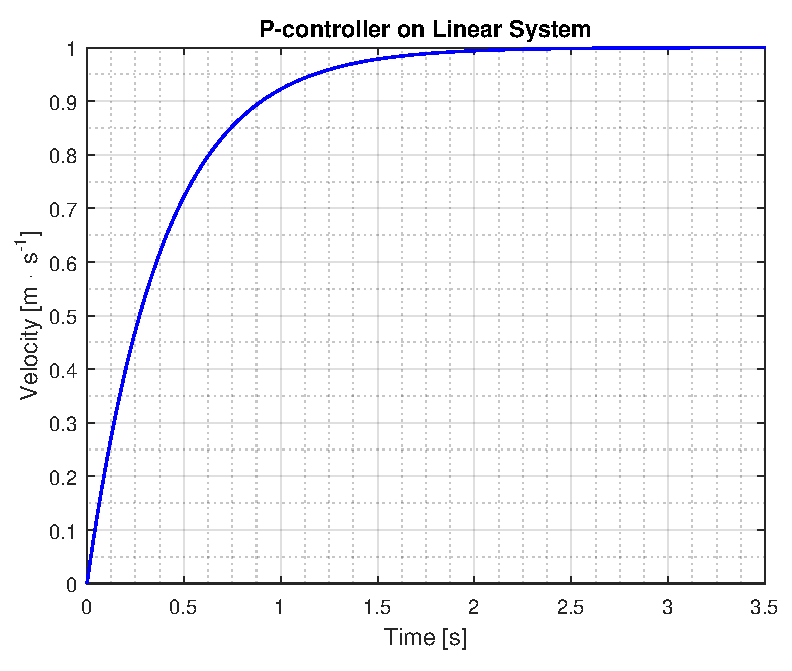
\includegraphics[width=.6\textwidth]{figures/ZstepPcontrolLinear.pdf}
	\caption{Step response of the linear transfer function with a P-controller with a gain of $-200$.}
	\label{fig:ZstepPcontrolLinear}
\end{figure}

However a P-controller does not account for input disturbances, and neither does the integrator in the plant. Therefore, if the equilibrium speed of the rotors has an offset under some flight conditions, this error will not be accounted for.\fxnote{further explanation and formulas are needed here}
To see this effect, the P-controller is tested on the nonlinear model with an added difference of \SI{5}{rad \cdot s^{-1}} in each of the 4 needed equilibrium speeds in the model. The simulation is seen below in \autoref{fig:ZstepPcontrolNonlinear}, where the reference input is subjected to a step of \SI{1}{m \cdot s^{-1}}, however, the velocity stabilizes instead at \SI{0.9}{m \cdot s^{-1}}, revealing a steady state error.

\begin{figure}[H]
	\centering
	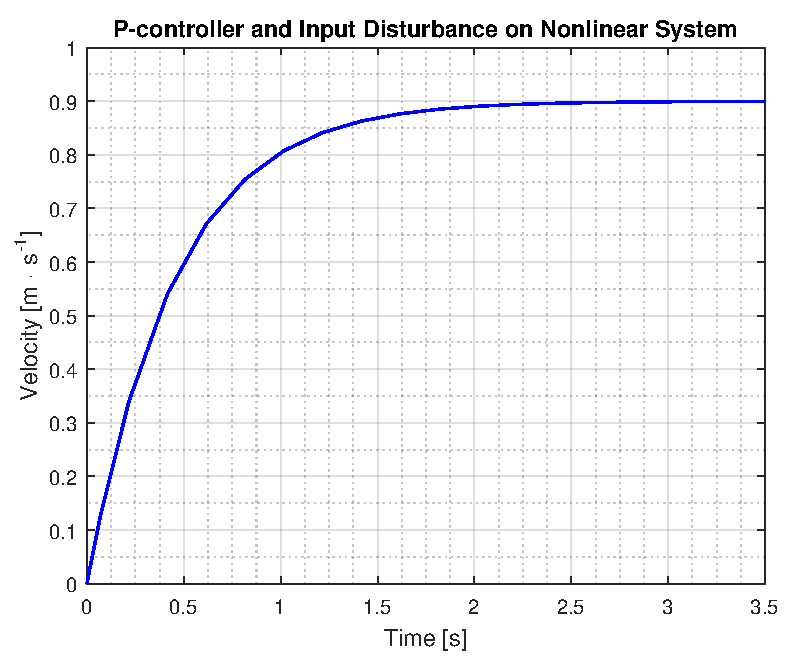
\includegraphics[width=.6\textwidth]{figures/ZstepPcontrolNonlinear.pdf}
	\caption{Step response of the nonlinear transfer function with a P-controller with a gain of $-200$.}
	\label{fig:ZstepPcontrolNonlinear}
\end{figure}
%
%In order to remove the steady state error an integrator is introduced to the controller. 

The plant is a type 1 system and steady state error is handled by the naturally occurring integrator within the plant. However, due to input disturbances a steady state error will be present in the output of the closed loop. This can be explained by the following derivations.   

\begin{figure}[H]
	\centering
	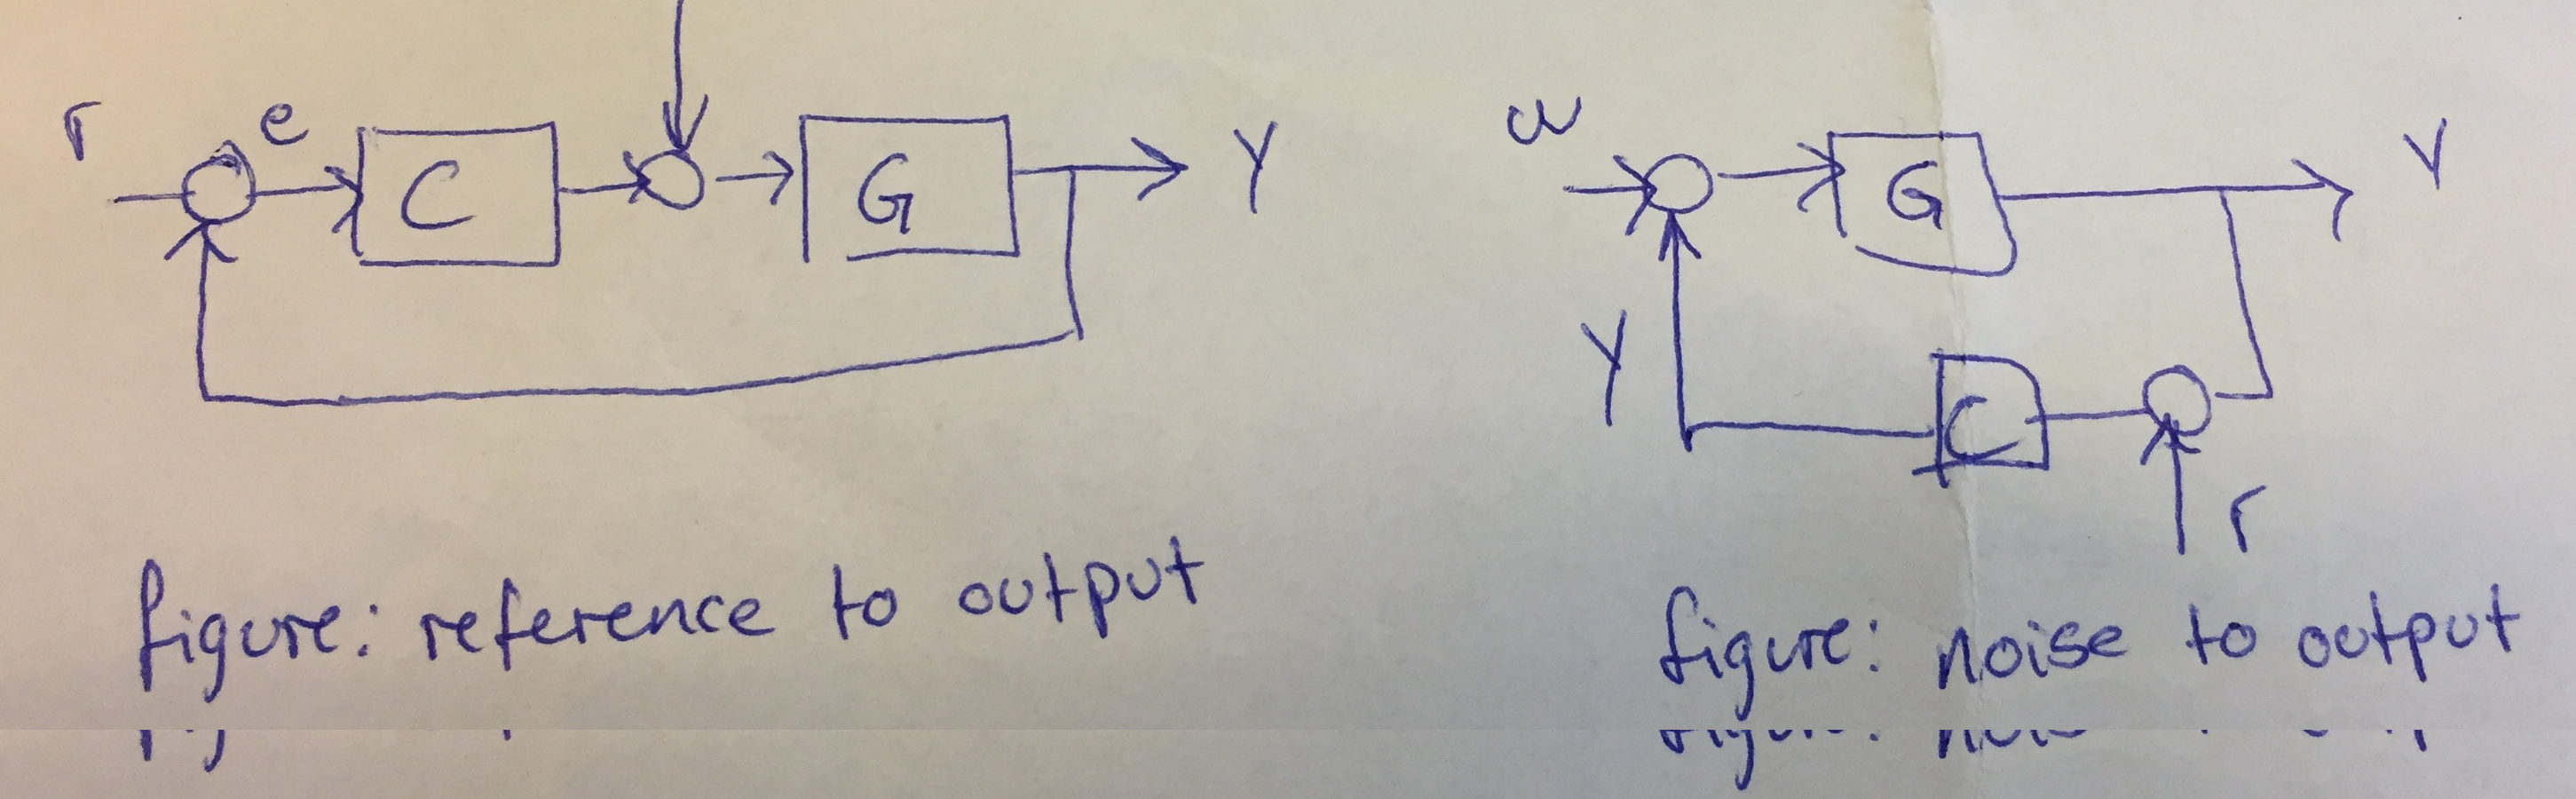
\includegraphics[width=.6\textwidth]{figures/inputdisturbance.png}
	\caption{Feedback loops including input disturbance.}
	\label{fig:rootLocusOfZwithPI}
\end{figure}\fxnote{dnt draw the rightmost figure}
A transfer function for the closed loop from disturbance to output is expressed as
\begin{align}
H=\frac{G}{1+CG}
\end{align}  
The plant is replaced with an integrator only. To show the present steady state error, the DC gain is considered.
%\begin{align}
%H\olestreg{P=\frac{1}{s}}=\frac{1}{S+C} \Rightarrow \lim_{s \to 0} H(s)\olestreg{P=\frac{1}{s}}= \frac{1}{C} \label{eq:dc_sse}
%\end{align}
\begin{where}
\va{H_{\mathrm{P}}}{is the transfer function, where the plant is an integrator}{1}
\end{where}
From \autoref{eq:dc_sse} it is clearly seen that a steady state is present and an increasing controller gain will decrease the error.
Adding an integrator to the controller, the DC gain is given as:
%\begin{align}
%H(s)\olestregTo{P=\frac{1}{s}}{I=frac{1}{s}} =\frac{1+s}{s^2+1} \Rightarrow \  \lim_{s \to 0} H(s)\olestreg{P=\frac{1}{s}} = 1 \label{eq:dc}
%\end{align}
\begin{where}
\va{H_{\mathrm{PI}}}{is the transfer function, where the plant and controller are both integrators}{1}
\end{where}
From \autoref{eq:dc} it is seen that no steady state error is eliminated. 
An integrator is therefore included in the control design. 

The root locus of the system, which now contains two poles in zero, will branch along the imaginary axis. To avoid oscillations the two loci are attracted by the use of a zero, placed on the left real axis as seen in \autoref{fig:rootLocusOfZwithPI}.

\begin{figure}[H]
	\centering
	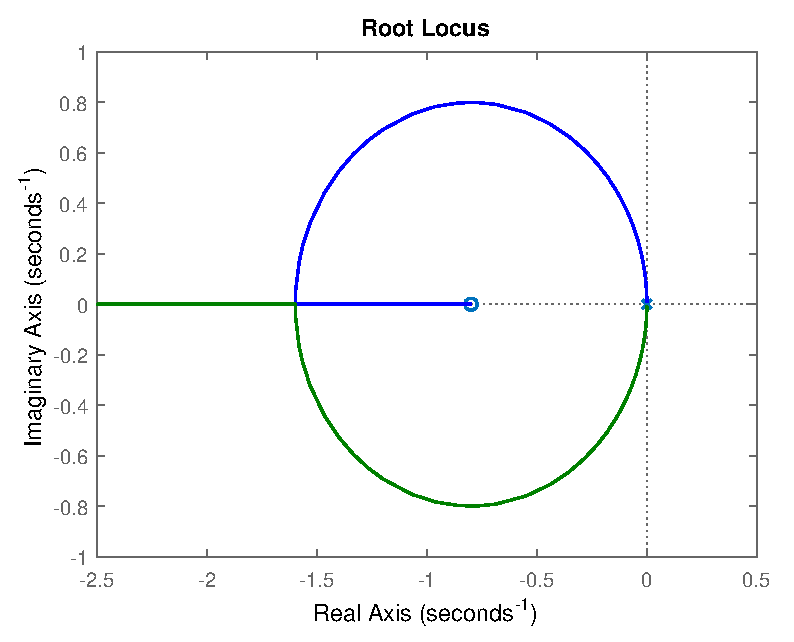
\includegraphics[width=.6\textwidth]{figures/rootLocusOfZwithPI.pdf}
	\caption{Root locus of the system with PI control. The zero is placed in (0,-0.8).}
	\label{fig:rootLocusOfZwithPI}
\end{figure}

The zero is placed and the gain is scaled to achieve a good rise time with a reasonable control action while still keeping the zero far enough from the poles, such that the integrator is not cancelled. The zero is placed in -0.8 on the real axis and with a gain of -201. The step response of the linear system with the PI controller is seen on \autoref{fig:stepOfZwithPI}.

\begin{figure}[H]
	\centering
	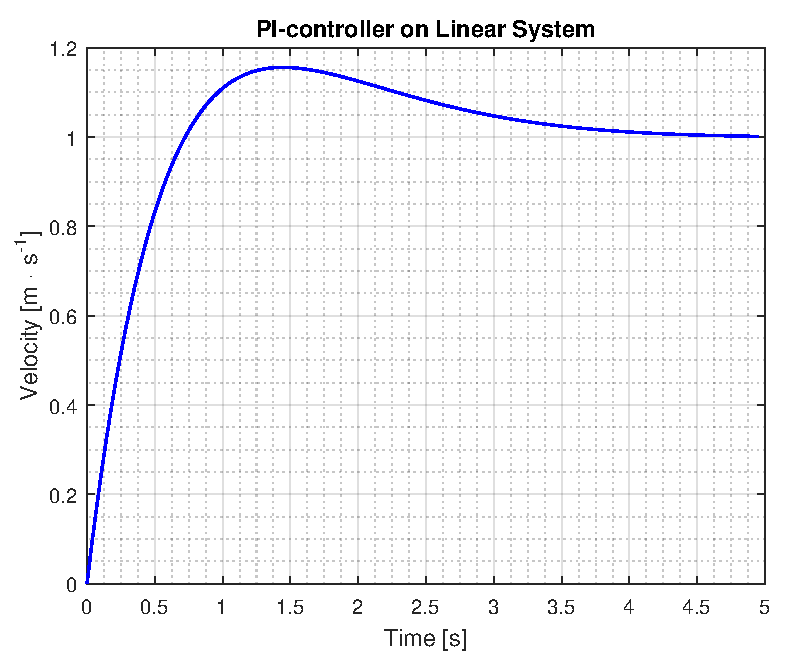
\includegraphics[width=.6\textwidth]{figures/stepOfZwithPI.pdf}
	\caption{Step response of the linear system with PI control.}
	\label{fig:stepOfZwithPI}
\end{figure}

\fxnote{simulation in nonlinear model}

